\subsubsection{Aufzeichnung und Analyse der ICMP requests und replys}

    \subsubsubsection{Fabliches Markieren von Bestandteilen der Paketinhalten}
        \textbf{Request}
        \begin{figure}[H]
            \centering
            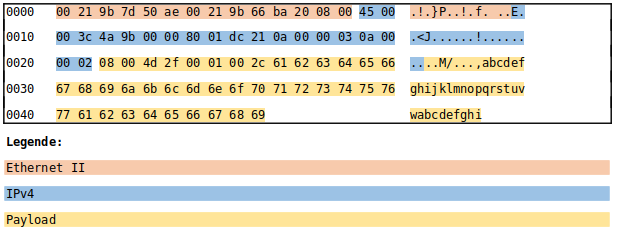
\includegraphics[width=\textwidth]{2_2/a_request.png}
            \source{Wireshark Mitschnitt von ping request}{eigene Zusammenstellung}{}
        \end{figure}
        \textbf{Reply}
        \begin{figure}[H]
            \centering
            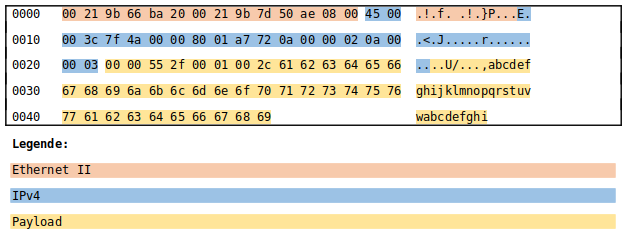
\includegraphics[width=\textwidth]{2_2/a_reply.png}
            \source{Wireshark Mitschnitt von ping reply}{eigene Zusammenstellung}{}
        \end{figure}

    \subsubsubsection{Ermittlung der WS1-IP und des dazugehörigen Hexadezimalcode im IP-Header}
        \textbf{IP Header}
        \begin{figure}[H]
            \centering
            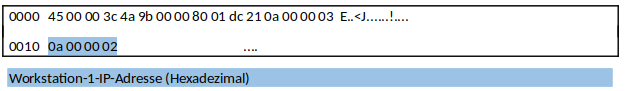
\includegraphics[width=\textwidth]{2_2/b_IP-Header.png}
            \source{IP Header}{eigene Zusammenstellung}{}
        \end{figure}

    \subsubsubsection{Bestimmung der MAC und des NIC}
        \begin{figure}[H]
            \centering
            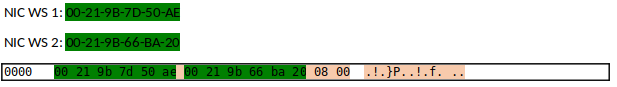
\includegraphics[width=\textwidth]{2_2/c_MAC_NIC.png}
            \source{Wireshark Mitschnitt von ping request}{eigene Zusammenstellung}{}
        \end{figure}

\subsection{Aufzeichnung der Protokollübertragung von hallo.htm zur WS2}
    \subsubsubsection{Header und Payload jeder Protokollschicht und Zuordnung zu OSI Schichten}
        \textbf{HTTP-Request}
        \begin{figure}[H]
            \centering
            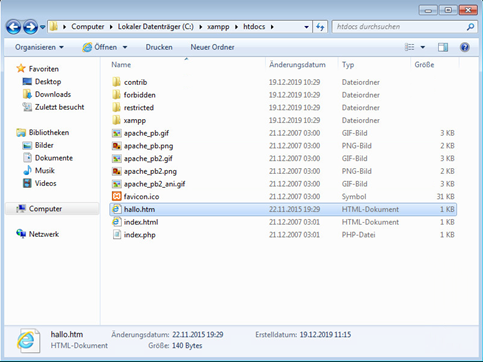
\includegraphics[width=\textwidth]{2_3/1.png}
            \source{Ethernet II (Schicht 2)}{eigene Zusammenstellung}{}
        \end{figure}
        \begin{figure}[H]
            \centering
            \includegraphics[width=\textwidth]{2_3/2.png}
            \source{IPv4 (Schicht 3)}{eigene Zusammenstellung}{}
        \end{figure}
        \begin{figure}[H]
            \centering
            \includegraphics[width=\textwidth]{2_3/3.png}
            \source{TCP (Schicht 4)}{eigene Zusammenstellung}{}
        \end{figure}
        \begin{figure}[H]
            \centering
            \includegraphics[width=\textwidth]{2_3/4.png}
            \source{HTTP}{eigene Zusammenstellung}{}
        \end{figure}
        \textbf{HTTP-REsponse}
        \begin{figure}[H]
            \centering
            \includegraphics[width=\textwidth]{2_3/5.png}
            \source{Ethernet II (Schicht 2)}{eigene Zusammenstellung}{}
        \end{figure}
        \begin{figure}[H]
            \centering
            \includegraphics[width=\textwidth]{2_3/6.png}
            \source{IPv4 (Schicht 3)}{eigene Zusammenstellung}{}
        \end{figure}
        \begin{figure}[H]
            \centering
            \includegraphics[width=\textwidth]{2_3/7.png}
            \source{TCP (Schicht 4)}{eigene Zusammenstellung}{}
        \end{figure}
        \begin{figure}[H]
            \centering
            \includegraphics[width=\textwidth]{2_3/8.png}
            \source{HTTP}{eigene Zusammenstellung}{}
        \end{figure}
        \begin{figure}[H]
            \centering
            \includegraphics[width=\textwidth]{2_3/9.png}
            \source{Payload}{eigene Zusammenstellung}{}
        \end{figure}

    \subsubsubsection{Verhältnis Payload zur Paketgröße nach DoD-Modell}

        \textbf{Request}
        \begin{longtable}{l|c|l|c}
    \hline
    Schicht & Größe in Byte & Protokoll & \makecell[l]{Verhältnis Payload \\zu Paketgröße}
    \\\hline
    Application & 519 & Data (HTTP) & 90,58 \%
    \\\hline
    Host-to-Host & 20 & Header (TCP) & -
    \\\hline
    Host-To-Host Gesamt & 539 & Data (HTTP + Payload + TCP) & 94,07 \%
    \\\hline
    Internet & 20 & Header (IPv4) & -
    \\\hline
    Internet Gesamt & 559 & Data (HTTP + Payload + TCP + IPv4) & 97,56 \%
    \\\hline
    Network-Access & 14 & Header (Ethernet) & - 
    \\\hline
    Paket Gesamt & 573 & Data (gesamt) & 100 \%

\end{longtable}
        \vspace{1cm}
        \textbf{Response}
        \begin{longtable}[width=\textwidth]{l|c|l|c}
    \hline
    Schicht & Größe in Byte & Protokoll & \makecell[l]{Verhältnis Payload \\zu Paketgröße}
    \\\hline
    Application & 444 & Data (HTTP + Payload) & 89,14 \%
    \\\hline
    Host-to-Host & 20 & Header (TCP) & -
    \\\hline
    Host-To-Host Gesamt & 464 & Data (HTTP + Payload + TCP) & 93,17 \%
    \\\hline
    Internet & 20 & Header (IPv4) & -
    \\\hline
    Internet Gesamt & 484 & Data (HTTP + Payload + TCP + IPv4) & 97,19 \%
    \\\hline
    Network-Access & 14 & Header (Ethernet) & -
    \\\hline
    Paket Gesamt & 498 & Data (gesamt) & 100 \%
    \\
    \caption{Payload der Response}
\end{longtable}

    \subsubsubsection{Anteil der Nutzdaten zum Frame für den Request und den Response}
        \textbf{Request}\\
        Frame: 573 Bytes \\
        HTML: 0 Bytes\\
        Anteil: 0 \%\\
        \textbf{Response}\\
        Frame: 498 Bytes\\
        HTML: 133 Bytes\\
        Anteil: 26,7 \%

\subsubsection{Umstellung von IPv4 auf IPv6}
    \begin{figure}[H]
        \centering
        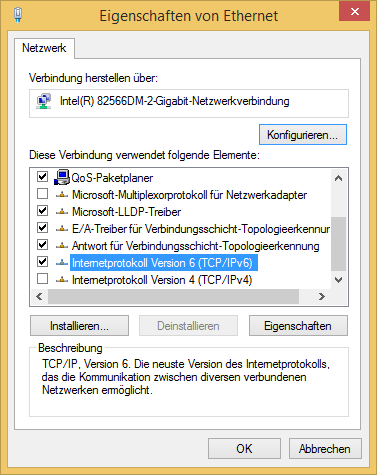
\includegraphics[width=0.5\textwidth]{2_2_3/umstellung_ipv4_ipv6.png}
        \source{Umstellung von IPv4 auf IPv6}{Screenshot}{}
    \end{figure}

    \subsubsubsection{Ausführung des Befehls ipv6 if}

    \begin{figure}[H]
        \centering
        \includegraphics[width=0.5\textwidth]{2_2_3/2.png}
        \source{Ausführung des Befehls ipv6 if}{Screenshot}{}
    \end{figure}

    \subsubsubsection{Testen der Verbindung mit ping, Ermittlung des korrektem Befehls}

    \begin{figure}[H]
        \centering
        \includegraphics[width=0.5\textwidth]{2_2_3/3.png}
        \source{Ausführen eines Pings auf eine IPv6}{Screenshot}{}
    \end{figure}

    \subsubsubsection{Testen der Aufzeichnung der Kommunikationsbeziehung mit Wireshark und die Unterschiede zu 2.2.1.1}
        \begin{figure}[H]
        \centering
        \includegraphics[width=0.5\textwidth]{2_2_3/4.png}
            \source{Mitschnitt via Wireshark}{Screenshot}{}
        \end{figure}

        \begin{figure}[H]
        \centering
        \includegraphics[width=0.5\textwidth]{2_2_3/5.png}
            \source{Mitschnitt via Wireshark}{Screenshot}{}
        \end{figure}

        \textbf{Unterschiede zu 2.2.1.1}
        \begin{itemize}
            \item Bei IPv6 ist IP-Header ist größer, da dieser die längeren IPv6 Adressen enthält
            \item Checksum im Payload hat sich verändert
            \item Bei IPv4 gibt es zwei Identifier (BE \& LE), bei IPv6 nur einen
            \item Bei IPv4 gibt es zwei Sequence numbers (BE \& LE), bei IPv6 nur eine sequence (number)
            \item Bei IPv4 gibt es eine “Time to live”, bei IPv6 heißt diese nun “Hop limit”
        \end{itemize}

    \subsubsubsection{Testen einer Ordnerfreigabe zur WS2}
        
        \begin{figure}[H]
        \centering
        \includegraphics[width=0.5\textwidth]{2_2_3/6.png}
            \source{Eigenschaften der Freigabe}{Screenshot}{}
        \end{figure}

        \begin{figure}[H]
        \centering
        \includegraphics[width=0.5\textwidth]{2_2_3/7.png}
            \source{Erweiterte Freigabe}{Screenshot}{}
        \end{figure}

        \begin{figure}[H]
        \centering
        \includegraphics[width=0.5\textwidth]{2_2_3/8.png}
            \source{Berechtigungen für die Freigabe}{Screenshot}{}
        \end{figure}

        \begin{figure}[H]
        \centering
        \includegraphics[width=0.5\textwidth]{2_2_3/9.png}
            \source{Bearbeiten der Sicherheit der Freigabe}{Screenshot}{}
        \end{figure}

        \begin{figure}[H]
        \centering
        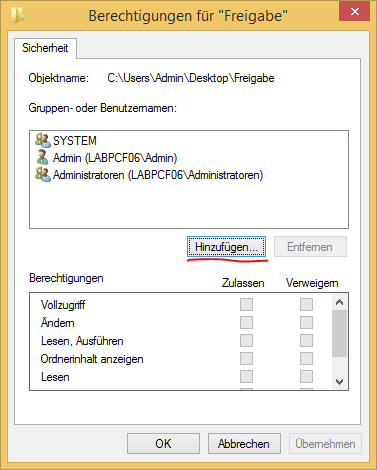
\includegraphics[width=0.5\textwidth]{2_2_3/10.png}
            \source{Berechtigungen hinzufügen}{Screenshot}{}
        \end{figure}

        \begin{figure}[H]
        \centering
        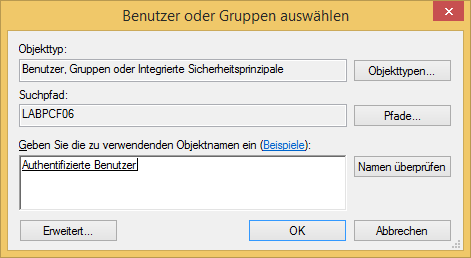
\includegraphics[width=0.5\textwidth]{2_2_3/11.png}
            \source{Einstellen der Bruntzergruppen}{Screenshot}{}
        \end{figure}

        \begin{figure}[H]
        \centering
        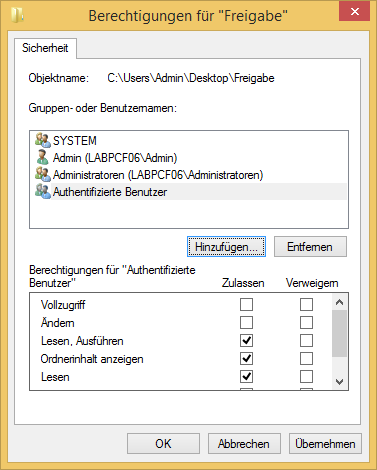
\includegraphics[width=0.5\textwidth]{2_2_3/12.png}
            \source{Berechtigungen für Freigabe}{Screenshot}{}
        \end{figure}

        \begin{figure}[H]
        \centering
        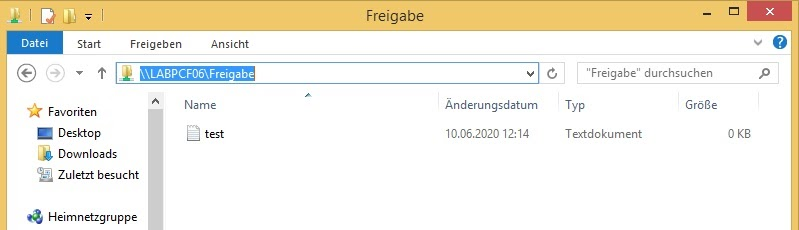
\includegraphics[width=0.5\textwidth]{2_2_3/13.png}
            \source{Anzeige des Freigegebenen Dokuments auf WS1}{Screenshot}{}
        \end{figure}